%
%                       This is a basic LaTeX Template
%                       for the Informatics Research Review

\documentclass[a4paper,11pt]{article}
% Add local fullpage and head macros
\usepackage{head,fullpage}     
% Add graphicx package with pdf flag (must use pdflatex)
\usepackage[pdftex]{graphicx}  
% Better support for URLs
\usepackage{url}
% Date formating
\usepackage{datetime}

\newdateformat{monthyeardate}{%
  \monthname[\THEMONTH] \THEYEAR}

\parindent=0pt          %  Switch off indent of paragraphs 
\parskip=5pt            %  Put 5pt between each paragraph  
\Urlmuskip=0mu plus 1mu %  Better line breaks for URLs


%                       This section generates a title page
%                       Edit only the following three lines
%                       providing your exam number, 
%                       the general field of study you are considering
%                       for your review, and name of IRR tutor

\newcommand{\examnumber}{s2517285}
\newcommand{\field}{Edge Computing Offloading in Internet of Things: Experimental Designs and Configurations}
\newcommand{\supervisor}{My IRR Tutor}

\begin{document}
\begin{minipage}[b]{110mm}
        {\Huge\bf School of Informatics
        \vspace*{17mm}}
\end{minipage}
\hfill
\begin{minipage}[t]{40mm}               
        \makebox[40mm]{
        
\includegraphics[width=40mm]{crest.png}}
\end{minipage}
\par\noindent
    % Centre Title, and name
\vspace*{2cm}
\begin{center}
        \Large\bf Informatics Research Review \\
        \Large\bf \field
\end{center}
\vspace*{1.5cm}
\begin{center}
        \bf \examnumber\\
        \monthyeardate\today
\end{center}
\vspace*{5mm}

%
%                       Insert your abstract HERE
%                       
\begin{abstract}
        The abstract is a short concise outline of your 
        project area, {\bf of no more than 100 words}.
\end{abstract}

\vspace*{1cm}

\vspace*{3cm}
Date: \today

\vfill
{\bf Supervisor:} \supervisor
\newpage

%                                               Through page and setup 
%                                               fancy headings
\setcounter{page}{1}                            % Set page number to 1
\footruleheight{1pt}
\headruleheight{1pt}
\lfoot{\small School of Informatics}
\lhead{Informatics Research Review}
\rhead{- \thepage}
\cfoot{}
\rfoot{Date: \date{\today}}
%

\section{Introduction}

%物联网的发展
Internet of Things (IoT) means that the objects around people can communicate with each other and cooperate to achieve the common goals, which has great potential for both private and business uses \cite{iot}. Most tasks handled by devices in IoT tend to be delay-sensitive, which also generates a mount of data nearly 49 EB \cite{Distributed_Offloading_in_Overlapping_Areas}. However, the IoT devices are usually limited in terms of memory, battery life, and computing power \cite{Internet_of_Things_offloading_Ongoing_issues, A_Cooperative_Partial_Computation_Offloading_Scheme_for_Mobile_Edge}. Hence, it is impossible to process all the application tasks in local devices and meanwhile satisfy all the performance requirements \cite{Distributed_Offloading_in_Overlapping_Areas}. As a consequence, computation offloading is applied to solve this problem. \newline\newline
In tradition, cloud computation integrates with the Internet of Things since cloud server. Unlike IoT, the storage and computation power provided centrally by the cloud server is almost unlimited, which corresponds to the disadvantages of IoT \cite{cloud_advatange,cloud_central}. Hence, cloud computing can help IoT devices to complete their computation tasks with high performance. However, for IoT devices it is an obstacle to obtain stable and acceptable network performance to reach the cloud \cite{cloud_advatange_and_problem}. Additionally, the cloud have to be challenged by reliability problem since the devices may fail or become inaccessible \cite{cloud_advatange_and_problem}. Unfortunately, the extensive scale of the resultant system, stemming from interactions with a significant number of devices, renders the rising requirements for storage capacity and computational power in subsequent processing progressively difficult to meet \cite{cloud_advatange_and_problem}. Therefore, edge computing is introduced to address the issues of the IoT and the cloud. \newline\newline
Edge Computing (EC), also named Mobile Edge Computing (MEC), provides cloud computing capabilities within the Radio Access Network close to mobile users \cite{EC_definition}. Comparing with the cloud computing, edge computing can compute in the real-time because the edge server are closer to the users \cite{edge_advantage_archetecture}. Moreover, edge computing doesn't need to upload the data to the cloud computing center and reduce the load on the network bandwidth, which lowers the cost and the network bandwidth pressure \cite{edge_advantage_archetecture}. Many algorithm has been designed to optimize the task offloading problem in IoT applications based on edge computing. Nevertheless, these algorithms shown high performance have not been systematically compared to come to a conclusion about the best algorithm. One of the reasons is the experimental designs and configurations for each algorithm is extremely different. Consequently, it is difficult to get an objective comparison. \newline\newline
As edge computing plays a significant role in coordinating the work between IoT devices, it is necessary to design optimization algorithms to enhance the functionality of IoT through the utilization of Edge Computing characteristics. Quantities of optimization algorithms have been proposed and implemented, however, it is impossible to compare their performance due to the difference between system models (edge computing models). There are several important components can be used to build different kinds of edge computing models for IoT devices, which may have a great impact on the performance of the algorithms on the edge computing. Hence, this review will summarize the designs or configurations for the IoT application based on edge computing. It is noted that the pattern mentioned only including cloud server, edge server and objective function.\newline\newline
To address the problem of differences in edge computing system models that result in incomparability, this article will attempt to answer the following questions:
        \begin{quote}
                1. What are the main differences between different system models? How those affect the performance of the algorithms?
        \end{quote}
        \begin{quote}
                2. Why the designers choose such configurations? What's the pros and cons?
        \end{quote}
        \begin{quote}
                3. Based on questions 1 and 2, what designs or configurations should be considered when applying optimization problems?
        \end{quote}
\noindent The section 2 will focus on the cloud computing component in the EC designs. Additionally, in section 3 the full offloading and partial offloading will be discussed. Last but not least, the section 4 will study on the different objective function chosen by the EC system models.
        

% and attempt to classify the models by finding similar configurations across the models. It should be noted that the pattern mentioned only including cloud server, edge server and objective function. For the similar models, their difference also will be discussed in the review. Additionally, the second question answered is the reason why these papers design such models and what is the benefit of the models. Furthermore, based on the results above, the review will try to derive a conclusion: What model should be employed for the implementation and comparison of existing algorithms.



% 许多算法被应用,但是他们的实验配置不同,难以比较

% 本文对不同的实验配置进行总结和介绍(架构不同、设备的不同),为什么他们要选择这样的配置,并尝试找出几种模式

% 1. 系统和问题的模型有哪些?他们是否有相似的模式,以及这些相似的模式中的每个模型的不同之处
% 2. 为什么要选这样的模型?这样的模式有什么好处
% 3. 基于1和2,找出应该使用什么模型来实现和比较已有的算法

%cloud server, edge computing and cost function
\section{Literature Review}
\subsection{Cloud Computing components}
Though the main conception discussed in this review is edge computing, it doesn't mean that the cloud components should be excluded from the edge computing models. 
% 什么时候选择有云服务器
% 云服务器的作用
% 什么时候把任务卸载到云服务器
% 总结:当前比较流行的是传统的云计算,现在的模式是边缘计算处理一些,再让云计算处理一些 \cite{why_cloud}. 但是考虑云计算的话模型会变得更复杂,模型需要考虑什么时候,把什么任务,由谁交给云计算处理,因此,如果只是研究edge computing的算法的话,不考虑云计算比较好;但如果更考虑现实的应用的话,需要考虑云计算

\subsection{Offloading Strategies}
Since the IoT devices have limited computation and energy resources, they can hardly satisfied the complicated tasks required by the IoT service. Therefore, the goal of the task offloading is to gain computation capability without using more energy-cost devices \cite{aim_offloading}. The offloading strategies can be separated into two categories: full offloading and partial offloading strategies. Full offloading strategy means offloading the task all to the edge computing server or cloud server. On the contrary, the partial offloading strategy is aimed at dividing tasks into two parts, one part is executed on the local machine while the other part is offloaded to the edge or cloud server \cite{full_partial}. 

\begin{figure}[h]
        \centering
        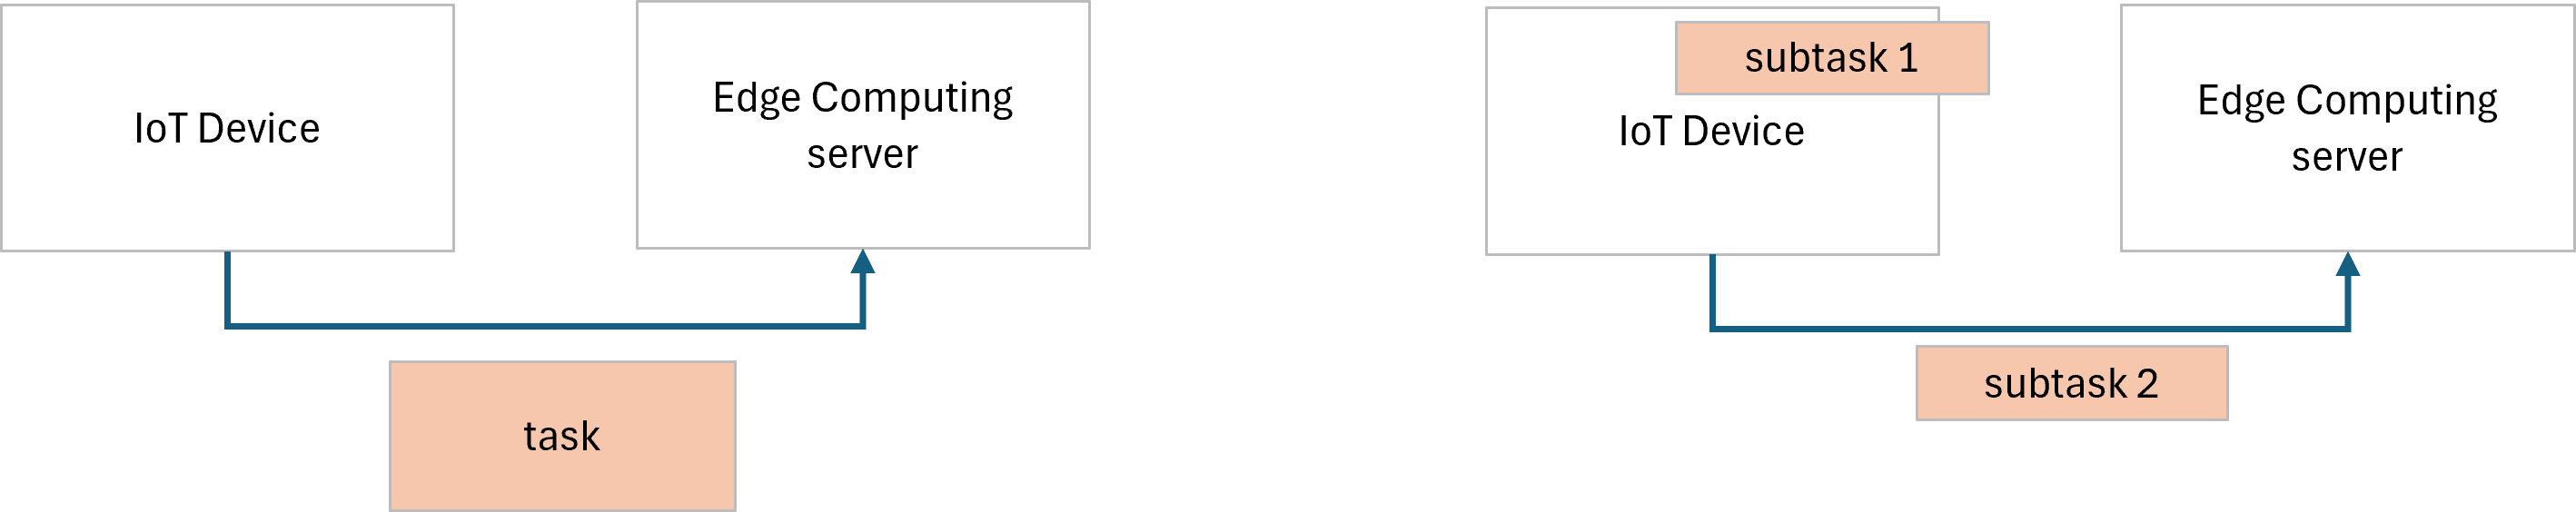
\includegraphics[width=0.8\textwidth]{offloading.png}
        \caption{Full offloading strategy VS partial offloading strategy}
\end{figure}
Ning and te.al suggests that one factor that affects the choice of different strategies is the type of the applications \cite{A_Cooperative_Partial_Computation_Offloading_Scheme_for_Mobile_Edge}. For example, if the input data of the application is privacy information, the tasks should be partial offloaded. Another important factor that influences the strategy is the ability of offloading, due to some part of the tasks shouldn't be offloaded \cite{A_Cooperative_Partial_Computation_Offloading_Scheme_for_Mobile_Edge}. On the condition that the task is allowed to be divided, for the reason of optimizing user's energy conservation, partial offloading strategy has a higher priority \cite{save_energy}. However, the offloading becomes more complicated when partial offloading strategy is considered, for the reason that the task relevance, characteristics and segmentation have to be concentrated \cite{user_central}. 
% xx文章选择了哪种卸载,具体如何建模的,以及选择这种卸载的理由
% 部分卸载有什么优点、缺点
% 怎么划分子任务,将子任务部分卸载
% 卸载的第二种分类:如何卸载到多个edge server,什么时候卸载到云服务器(从用户还是从edge server)
% 总结

\subsection{Objective Functions}
% 有哪些objective functions
% 为什么选择这个objective functions
% 哪个更好,或者在比较的时候要选择哪个更加普遍性的objective function

\subsection{Other Difference}
% 其他的不同


\section{Summary \& Conclusion}


%                Now build the reference list
\bibliographystyle{unsrt}   % The reference style
%                This is plain and unsorted, so in the order
%                they appear in the document.


\small
\bibliography{main}       % bib file(s).

\end{document}

